\chapter{Operadores de Koopman cerca de ciclos límite}

Los capítulos anteriores prepararon de manera natural el terreno para un cambio de perspectiva especialmente profundo. La teoría de Floquet mostró que la periodicidad puede reorganizarse en una parte exponencial efectiva y una parte periódica moduladora. Los \emph{embeddings} de Carleman mostraron que una dinámica no lineal polinomial puede desplegarse como una jerarquía lineal sobre una familia de monomios. Ambas teorías, cada una a su manera, sugieren una misma intuición: la dinámica puede volverse más transparente cuando se la traslada a un espacio ampliado donde ciertas estructuras se hacen explícitas.

La teoría de Koopman lleva esta intuición un paso más allá. En lugar de seguir directamente la evolución del estado, propone seguir la evolución de funciones del estado, es decir, de observables. La novedad conceptual es notable: aunque la dinámica en el espacio de estado sea no lineal, la evolución inducida sobre observables puede describirse mediante un operador lineal. Esta linealidad no aparece en un espacio de dimensión pequeña ni en una base predeterminada; aparece en un espacio funcional.

En el contexto de esta monografía, el interés de esta perspectiva se vuelve particularmente claro cerca de ciclos límite. Allí la dinámica posee una estructura periódica dominante, una fase natural a lo largo de la órbita y direcciones transversales asociadas a decaimientos o crecimientos modulados. La teoría de Koopman permite reorganizar todo ello en un lenguaje espectral sobre observables: aparecen funciones de fase, armónicos, exponentes transversales y familias de modos que recuerdan, pero ya no coinciden exactamente, con las estructuras vistas en Floquet.

El propósito de este capítulo será introducir esta perspectiva con la misma cautela pedagógica adoptada en capítulos anteriores. Primero prepararemos una lectura geométrica comparando modos lineales, modos de Floquet y observables no lineales; después formularemos la motivación conceptual: por qué conviene pasar de estados a observables y qué tipo de linealidad se obtiene con ello. Después presentaremos el operador y el generador de Koopman, y estudiaremos cómo emergen eigenfunciones de fase y armónicos en torno a un ciclo límite. Más adelante examinaremos la escalera espectral que aparece en sistemas periódicos, la geometría local en coordenadas tubulares, la conexión con observables armónicos y algunas advertencias prácticas sobre su aproximación computacional.

Leído en continuidad con Floquet y Carleman, el capítulo de Koopman no representa una ruptura, sino una culminación natural. Si Floquet reorganizaba la periodicidad y Carleman reorganizaba la no linealidad polinomial, Koopman reorganiza la dinámica desde el punto de vista más amplio de los observables. El cambio de enfoque es decisivo: ya no se trata solo de ampliar el espacio de estado, sino de elegir qué funciones del estado son las portadoras más transparentes de la estructura dinámica.


\section{De modos lineales a observables no lineales}

Antes de definir formalmente el operador de Koopman, conviene preparar la intuición geométrica que motiva su aparición. Una manera natural de hacerlo es comparar tres niveles de organización dinámica: los sistemas lineales invariantes en el tiempo, los sistemas lineales periódicos y los sistemas no lineales. En los tres casos aparece, de una u otra forma, la misma pregunta: ¿cómo se organiza una respuesta en componentes elementales?

En un sistema lineal invariante en el tiempo,
\begin{equation}
\dot{x}=Ax,
\label{eq:Koopman_LTI_intro_system}
\end{equation}
la respuesta se expresa, bajo condiciones apropiadas, como una suma de modos exponenciales,
\begin{equation}
x(t)=\sum_j c_j e^{\lambda_j t}v_j.
\label{eq:Koopman_LTI_intro_modes}
\end{equation}
Aquí los vectores \(v_j\) definen direcciones modales fijas, los exponentes \(\lambda_j\) determinan crecimiento, amortiguamiento u oscilación, y los coeficientes \(c_j\) dependen de la condición inicial. La geometría es relativamente simple: el espacio de estados se descompone en direcciones privilegiadas y cada una evoluciona con su propia ley exponencial.

En un sistema lineal periódico,
\begin{equation}
\dot{x}=A(t)x, \qquad A(t+T)=A(t),
\label{eq:Koopman_LTP_intro_system}
\end{equation}
la teoría de Floquet conserva la estructura exponencial, pero la reviste con una modulación periódica. La matriz fundamental puede escribirse como
\begin{equation}
\Phi(t)=P(t)e^{Rt},
\qquad P(t+T)=P(t).
\label{eq:Koopman_LTP_intro_floquet}
\end{equation}
Por ello, una componente modal típica adopta la forma
\begin{equation}
x_j(t)=e^{\mu_j t}p_j(t),
\qquad p_j(t+T)=p_j(t).
\label{eq:Koopman_LTP_intro_mode}
\end{equation}
La interpretación geométrica cambia: las direcciones modales ya no son rígidas, sino que respiran, giran o se deforman con el periodo del sistema. La periodicidad no destruye la lectura modal; la vuelve pulsante.

En un sistema no lineal,
\begin{equation}
\dot{x}=f(x),
\label{eq:Koopman_NL_intro_system}
\end{equation}
la situación cambia de manera más profunda. En general, no existe una descomposición global del espacio de estados en direcciones lineales fijas. Dos trayectorias que parten de regiones distintas pueden activar comportamientos cualitativamente diferentes; la dependencia respecto a las condiciones iniciales deja de ser una simple combinación lineal de modos. Sin embargo, la perspectiva de Koopman conserva una idea esencial: la posibilidad de describir la evolución mediante exponenciales, no ya en el espacio original de estados, sino en un espacio de observables.

Si \(g\) es un observable y \(\varphi^t\) es el flujo del sistema, el operador de Koopman actúa como
\begin{equation}
(U^t g)(x_0)=g(\varphi^t(x_0)).
\label{eq:Koopman_intro_operator_preview}
\end{equation}
Cuando existen eigenfunciones \(\phi_j\) tales que
\begin{equation}
U^t\phi_j(x_0)=e^{\lambda_j t}\phi_j(x_0),
\label{eq:Koopman_intro_eigen_preview}
\end{equation}
un observable físico puede escribirse, al menos local o formalmente, como
\begin{equation}
g(\varphi^t(x_0))
\approx
\sum_j c_j e^{\lambda_j t}\phi_j(x_0).
\label{eq:Koopman_intro_observable_expansion}
\end{equation}
La diferencia conceptual es importante. En el caso lineal, los coeficientes modales son proyecciones del estado inicial sobre direcciones fijas. En la perspectiva de Koopman, las amplitudes y fases modales se obtienen evaluando funciones del estado inicial. La sensibilidad a las condiciones iniciales no desaparece: queda codificada en los observables \(\phi_j(x_0)\).

De manera esquemática,
\begin{equation}
\begin{array}{lll}
\text{LTI:} &
x(t)=\displaystyle\sum_j c_j e^{\lambda_j t}v_j,
&
\text{direcciones modales fijas},
\\[2mm]
\text{LTP:} &
x(t)=\displaystyle\sum_j c_j e^{\mu_j t}p_j(t),
&
p_j(t+T)=p_j(t),
\\[2mm]
\text{No lineal/Koopman:} &
g(\varphi^t(x_0))\approx
\displaystyle\sum_j c_j e^{\lambda_j t}\phi_j(x_0),
&
\text{observables geométricos}.
\end{array}
\label{eq:Koopman_intro_comparison_table}
\end{equation}

La comparación anterior puede visualizarse observando una sola componente modal idealizada. La Figura~\ref{fig:lti-ltp-koopman-componentes} no representa tres simulaciones completas, sino tres formas elementales de organización de una respuesta: exponencial pura, exponencial periódicamente modulada y exponencial ponderada por un observable geométrico.

\begin{figure}[htbp]
\centering

\begin{tikzpicture}

\begin{groupplot}[
    group style={
        group size=1 by 3,
        vertical sep=1.15cm,
    },
    width=0.88\textwidth,
    height=4.0cm,
    xmin=0, xmax=20,
    grid=both,
    grid style={gray!20},
    major grid style={gray!35},
    minor tick num=1,
    xlabel={$t$},
    ylabel={componente},
    tick label style={font=\small},
    label style={font=\small},
    title style={align=center, font=\small\bfseries},
    legend style={
        font=\scriptsize,
        draw=none,
        fill=white,
        fill opacity=0.85,
        text opacity=1
    },
    samples=500,
    domain=0:20
]

% ------------------------------------------------------------
% Panel 1: LTI
% ------------------------------------------------------------
\nextgroupplot[
    title={\shortstack{Componente LTI:\\ modo exponencial con envolvente fija}},
    ymin=-1.1, ymax=1.1,
    legend pos=north east
]

\addplot[
    thick,
    BookGreen
]
{exp(-0.08*x)*cos(deg(2.0*x + 0.3))};

\addlegendentry{$e^{\sigma t}\cos(\omega t+\phi)$}

\addplot[
    dashed,
    thick,
    BookBrown
]
{exp(-0.08*x)};

\addlegendentry{$+e^{\sigma t}$}

\addplot[
    dashed,
    thick,
    BookBrown
]
{-exp(-0.08*x)};

\addlegendentry{$-e^{\sigma t}$}

% ------------------------------------------------------------
% Panel 2: LTP
% ------------------------------------------------------------
\nextgroupplot[
    title={\shortstack{Componente LTP:\\ exponencial revestida por modulación periódica}},
    ymin=-1.55, ymax=1.55,
    legend pos=north east
]

% p(t)=1+0.35 cos(0.9t)+0.15 sin(1.8t)
% y(t)=exp(-0.05t) p(t) cos(1.4t+0.1)

\addplot[
    thick,
    BookGreen
]
{exp(-0.05*x)*(1 + 0.35*cos(deg(0.9*x)) + 0.15*sin(deg(1.8*x)))*cos(deg(1.4*x + 0.1))};

\addlegendentry{$e^{\mu t}p(t)\cos(\omega_F t)$}

\addplot[
    dashed,
    thick,
    BookBrown
]
{exp(-0.05*x)*(1 + 0.35*cos(deg(0.9*x)) + 0.15*sin(deg(1.8*x)))};

\addlegendentry{$+e^{\mu t}p(t)$}

\addplot[
    dashed,
    thick,
    BookBrown
]
{-exp(-0.05*x)*(1 + 0.35*cos(deg(0.9*x)) + 0.15*sin(deg(1.8*x)))};

\addlegendentry{$-e^{\mu t}p(t)$}

% ------------------------------------------------------------
% Panel 3: Koopman / sistema no lineal
% ------------------------------------------------------------
\nextgroupplot[
    title={\shortstack{Componente no lineal/Koopman:\\ exponencial ponderada por observables}},
    ymin=-0.95, ymax=0.95,
    legend pos=north east
]

% Real{ rho0 exp(j k theta0) exp((-sigma + j k omega)t)}
% = rho0 exp(-sigma t) cos(k omega t + k theta0)
% parameters: sigma=0.18, omega=1.4, k=3, theta0=0.4

\addplot[
    thick,
    BookGreen
]
{0.25*exp(-0.18*x)*cos(deg(3*1.4*x + 3*0.4))};

\addlegendentry{$\rho_0=0.25$}

\addplot[
    thick,
    BookBrown
]
{0.55*exp(-0.18*x)*cos(deg(3*1.4*x + 3*0.4))};

\addlegendentry{$\rho_0=0.55$}

\addplot[
    thick,
    BookRed
]
{0.90*exp(-0.18*x)*cos(deg(3*1.4*x + 3*0.4))};

\addlegendentry{$\rho_0=0.90$}

\end{groupplot}

\end{tikzpicture}

\caption{Lectura geométrica de una componente modal en tres niveles de organización dinámica. 
En un sistema LTI, una componente modal evoluciona como una exponencial oscilatoria con envolvente fija. 
En un sistema LTP, la exponencial de Floquet aparece revestida por una función periódica \(p(t)\), de modo que la envolvente respira con el periodo del sistema. 
En la perspectiva de Koopman para sistemas no lineales, la componente exponencial se conserva en el espacio de observables, pero su amplitud y fase dependen de la evaluación de una eigenfunción u observable geométrico en la condición inicial.}
\label{fig:lti-ltp-koopman-componentes}
\end{figure}



Esta comparación permite ver la continuidad conceptual: los sistemas lineales organizan la respuesta mediante exponentes y direcciones; los sistemas periódicos mediante exponentes y formas periódicas; los sistemas no lineales mediante exponentes y observables. La linealidad no desaparece por completo, sino que se desplaza hacia un espacio funcional.

\IdeaClave{Koopman no elimina la sensibilidad a condiciones iniciales; la codifica en observables. La respuesta de un sistema no lineal puede entenderse, localmente, como una superposición de exponenciales cuyas amplitudes y fases dependen de funciones geométricas evaluadas en el estado inicial.}

Cerca de un ciclo límite, esta lectura adquiere una forma especialmente transparente. Si \(\theta\) representa la fase sobre el ciclo y \(\rho\) una coordenada transversal, aparecen observables locales del tipo
\begin{equation}
\phi_{k,m}(\rho,\theta)=\rho^m e^{jk\theta}.
\label{eq:Koopman_intro_limit_cycle_observable}
\end{equation}
Su evolución combina rotación armónica y decaimiento transversal:
\begin{equation}
\phi_{k,m}(t)=
e^{(-m\sigma+jk\omega)t}\phi_{k,m}(0).
\label{eq:Koopman_intro_limit_cycle_evolution}
\end{equation}
Así, la fase inicial, la distancia al ciclo y la frecuencia fundamental quedan incorporadas en una misma descripción modal. En este sentido, Koopman ofrece una lectura particularmente adecuada para la narrativa de esta monografía: Fourier organiza señales, Floquet organiza sistemas periódicos, Carleman organiza no linealidades algebraicas y Koopman organiza la dinámica no lineal desde sus observables.

Con esta lectura geométrica en mente, podemos pasar ahora a la motivación formal del capítulo: por qué conviene cambiar el objeto dinámico de estudio y seguir funciones del estado en lugar de seguir únicamente el estado mismo.

\section{Motivación: de estados a observables}

La formulación habitual de un sistema dinámico parte del estado. Se escribe una ecuación del tipo
\begin{equation}
\dot{x}=f(x),
\label{eq:Koopman_motivation_state_dynamics}
\end{equation}
y se estudia cómo evoluciona \(x(t)\) en el espacio de estados. Esta perspectiva es natural, pero no siempre es la más reveladora. En muchos problemas, y especialmente cerca de ciclos límite, la estructura relevante no reside únicamente en la trayectoria del estado, sino en cómo ciertas funciones del estado --amplitudes, fases, combinaciones modales, salidas medibles-- evolucionan a lo largo del flujo.

La teoría de Koopman parte precisamente de esa observación. En lugar de concentrarse exclusivamente en la evolución de \(x(t)\), considera la evolución de observables
\begin{equation}
g:X\to\mathbb{C},
\label{eq:Koopman_motivation_observable}
\end{equation}
donde \(X\) es el espacio de estados. Si \(\varphi^t(x)\) denota el flujo del sistema, entonces la evolución del observable viene dada por
\begin{equation}
g(x)\longmapsto g(\varphi^t(x)).
\label{eq:Koopman_motivation_flow_observable}
\end{equation}
La idea clave es que esta transformación es lineal respecto al observable \(g\), aunque la dinámica del estado sea no lineal.

\subsection{Por qué cambiar de objeto dinámico}

Este cambio de objeto dinámico tiene consecuencias profundas. La no linealidad puede hacer que el espacio de estados resulte difícil de organizar globalmente, especialmente cuando aparecen ciclos límite, cuencas, foliaciones de fase o estructuras transversales. Pero ciertas funciones del estado pueden capturar esas regularidades de manera mucho más directa. Una coordenada de fase, por ejemplo, puede evolucionar linealmente incluso cuando la trayectoria en el espacio original recorre una órbita geométricamente compleja.

Desde esta perspectiva, pasar de estados a observables no es un artificio, sino una decisión estructural. Se busca elegir funciones que hagan visible la organización interna del flujo. El problema ya no es solo describir dónde está el sistema en cada instante, sino identificar qué cantidades del sistema evolucionan de manera especialmente simple o especialmente reveladora.

\subsection{Relación con Carleman}

La conexión con el capítulo anterior es inmediata. En el \emph{embedding} de Carleman, la dinámica no lineal se reescribía como una jerarquía lineal sobre monomios del estado. Esa construcción puede leerse ahora como una primera incursión en el mundo de los observables: los monomios
\[
x^\alpha
\]
eran precisamente una familia especial de funciones del estado sobre las cuales la dinámica adquiría una forma lineal infinita-dimensional.

La teoría de Koopman conserva esta intuición, pero la amplía de manera decisiva. Ya no se limita a observables monomiales ni a sistemas polinomiales. La pregunta se vuelve mucho más general:
\begin{quote}
¿sobre qué espacio de observables la dinámica induce una evolución lineal útil?
\end{quote}
Carleman responde a esta pregunta con una elección algebraica muy concreta; Koopman la transforma en un principio operatorial.

\subsection{El tipo de linealidad que aparece}

Conviene subrayar desde el inicio que la linealidad de Koopman no es la linealidad habitual del espacio de estados. No significa que el sistema no lineal se convierta en un sistema lineal de dimensión finita en sus variables originales. Significa, más bien, que la composición con el flujo
\[
g\mapsto g\circ \varphi^t
\]
define una transformación lineal sobre observables. Es una linealidad funcional, no necesariamente una linealidad sobre coordenadas del estado.

Esta distinción es crucial. El precio de la linealidad es ahora el paso a un espacio funcional, potencialmente infinito-dimensional. Una vez más, la dificultad del problema no desaparece; se desplaza. Pero el desplazamiento puede ser extraordinariamente revelador, porque permite usar intuiciones espectrales y modales en contextos donde el estado mismo no ofrecía una estructura simple.


\Observacion{Conviene mantener desde ahora una cautela importante. El operador de Koopman no vive en el vacío: su significado analítico depende del espacio de observables que se elija. No es lo mismo trabajar con funciones continuas, suaves, cuadrado-integrables o analíticas. En esta monografía usaremos la teoría principalmente como una guía estructural cerca de ciclos límite, donde ciertas familias de observables —fase, armónicos e isostables— permiten organizar la dinámica de manera especialmente transparente.}

\subsection{Por qué los ciclos límite son un escenario privilegiado}

La vecindad de un ciclo límite es uno de los escenarios más fértiles para la teoría de Koopman. Allí coexisten, de manera natural, varios ingredientes que piden una descripción sobre observables:
\begin{itemize}
\item una fase que avanza regularmente a lo largo de la órbita;
\item direcciones transversales con decaimiento o crecimiento;
\item armónicos asociados a la periodicidad básica;
\item y observables físicos cuya respuesta se organiza alrededor de esa fase y de esos decaimientos.
\end{itemize}

En otras palabras, un ciclo límite ya trae consigo una estructura espectral embrionaria. Floquet la describía mediante exponentes y modulación periódica; Koopman permitirá describirla mediante eigenfunciones de fase y observables asociados. Esta es una de las razones por las que ambos enfoques están tan próximos en espíritu.

\subsection{La fase como primera pista}

Una manera muy simple de intuir la utilidad de Koopman cerca de un ciclo límite es pensar en la fase. Si \(\theta(x)\) representa una función de fase asintótica, entonces a lo largo del flujo del sistema se espera una evolución del tipo
\begin{equation}
\theta(\varphi^t(x))=\theta(x)+\omega t,
\label{eq:Koopman_motivation_phase}
\end{equation}
al menos módulo \(2\pi\). En términos del observable complejo
\begin{equation}
g(x)=e^{j\theta(x)},
\label{eq:Koopman_motivation_phase_observable}
\end{equation}
esto se convierte en
\begin{equation}
g(\varphi^t(x))=e^{j\omega t}g(x).
\label{eq:Koopman_motivation_phase_eigen}
\end{equation}
Aquí aparece ya una de las ideas fundamentales del capítulo: ciertos observables evolucionan simplemente por multiplicación exponencial. Esa es precisamente la señal de una eigenfunción del operador de Koopman.

\subsection{De periodicidad y no linealidad a estructura operatorial}

Leído en el contexto de esta monografía, el paso a Koopman puede resumirse así. El balance armónico hizo visible una estructura espectral en la respuesta periódica. Floquet mostró que la periodicidad lineal puede factorizarse y reorganizarse. Carleman mostró que una no linealidad polinomial puede desplegarse sobre monomios. Koopman toma estas intuiciones y las sitúa en un marco más general: la dinámica puede estudiarse como evolución lineal sobre funciones del estado.

Esta ampliación no borra las teorías anteriores; las contiene y las reorganiza. Los armónicos, los monomios, las fases y los decaimientos transversales aparecen ahora como piezas de una misma pregunta: qué observables hacen visible la estructura dinámica de la manera más transparente.

\subsection{Lo que sigue}

Con esta motivación en mente, el siguiente paso será definir de forma precisa el operador de Koopman y su generador. A partir de ahí podremos estudiar cómo surgen eigenfunciones, cómo se organiza el espectro cerca de un ciclo límite y cómo esta lectura se conecta con la fase, con Floquet y con las estructuras armónicas que han ido apareciendo a lo largo de toda la monografía.

\section{Operador y generador de Koopman}

La motivación del capítulo mostró que la teoría de Koopman propone cambiar el objeto dinámico de estudio: en lugar de seguir directamente la evolución del estado, se sigue la evolución de observables. Corresponde ahora formalizar esta idea.

\subsection{El flujo del sistema}

Consideremos un sistema dinámico autónomo
\begin{equation}
\dot{x}=f(x),
\label{eq:Koopman_operator_system}
\end{equation}
definido sobre un espacio de estados \(X\subseteq\mathbb{R}^n\), y sea
\begin{equation}
\varphi^t:X\to X
\label{eq:Koopman_operator_flow}
\end{equation}
su flujo, es decir, la aplicación que asigna a cada condición inicial \(x\in X\) el estado alcanzado en tiempo \(t\). Por definición,
\begin{equation}
\varphi^0(x)=x,
\qquad
\varphi^{t+s}(x)=\varphi^t(\varphi^s(x)).
\label{eq:Koopman_operator_semigroup_flow}
\end{equation}

La formulación habitual de la dinámica se concentra en el movimiento de \(x\) bajo \(\varphi^t\). La teoría de Koopman, en cambio, toma como objeto principal a una familia de observables
\begin{equation}
g:X\to\mathbb{C},
\label{eq:Koopman_operator_observable}
\end{equation}
y estudia cómo cambian dichas funciones al ser compuestas con el flujo.

\subsection{Definición del operador de Koopman}

Para cada \(t\ge 0\), el \emph{operador de Koopman} \(U^t\) actúa sobre observables según
\begin{equation}
(U^t g)(x)=g(\varphi^t(x)).
\label{eq:Koopman_operator_definition}
\end{equation}
Es decir, \(U^t g\) es el observable obtenido al evaluar \(g\) no en el estado actual \(x\), sino en el estado al que el sistema evoluciona después de un tiempo \(t\).

La idea es simple, pero de gran alcance. El operador \(U^t\) no actúa sobre el estado \(x\), sino sobre funciones del estado. A cada observable le asigna otro observable. La dinámica del sistema se traslada así desde el espacio de estados al espacio de funciones definidas sobre él.

\subsection{Linealidad del operador}

La propiedad más importante de \(U^t\) es su linealidad. Si \(g_1\) y \(g_2\) son observables y \(\alpha,\beta\in\mathbb{C}\), entonces
\begin{equation}
U^t(\alpha g_1+\beta g_2)
=
\alpha U^t g_1+\beta U^t g_2.
\label{eq:Koopman_operator_linearity}
\end{equation}
En efecto,
\begin{align}
(U^t(\alpha g_1+\beta g_2))(x)
&=
(\alpha g_1+\beta g_2)(\varphi^t(x)) \notag\\
&=
\alpha g_1(\varphi^t(x))+\beta g_2(\varphi^t(x)) \notag\\
&=
\alpha (U^t g_1)(x)+\beta (U^t g_2)(x).
\label{eq:Koopman_operator_linearity_proof}
\end{align}

Esta linealidad es la característica definitoria de la teoría. Aunque la dinámica del estado \(\dot{x}=f(x)\) sea no lineal, la evolución inducida sobre observables por composición con el flujo es lineal. Desde esta perspectiva, Koopman no linealiza el sistema en el espacio de estados, sino que traslada el problema a un espacio funcional donde la dinámica aparece como una familia de operadores lineales.

\subsection{Estructura de semigrupo}

Los operadores \(U^t\) heredan del flujo una estructura natural de semigrupo:
\begin{equation}
U^0=I,
\qquad
U^{t+s}=U^sU^t,
\label{eq:Koopman_operator_semigroup}
\end{equation}
donde \(I\) es el operador identidad sobre observables y la composición se entiende de derecha a izquierda. En efecto,
\begin{align}
(U^{t+s}g)(x)
&=
g(\varphi^{t+s}(x)) \notag\\
&=
g(\varphi^t(\varphi^s(x))) \notag\\
&=
(U^t g)(\varphi^s(x)) \notag\\
&=
(U^s(U^t g))(x).
\label{eq:Koopman_operator_semigroup_proof}
\end{align}
Como se trata de un flujo autónomo, los tiempos conmutan cuando ambos operadores están definidos, y también puede escribirse \(U^tU^s=U^sU^t=U^{t+s}\). Lo importante para lo que sigue es que la familia \(\{U^t\}_{t\ge 0}\) conserva, en el espacio de observables, la estructura temporal del flujo original.

Esta propiedad muestra que la familia \(\{U^t\}_{t\ge 0}\) juega, en el espacio de observables, un papel análogo al del flujo en el espacio de estados. La diferencia es que la evolución ahora se expresa mediante operadores lineales sobre funciones.

\subsection{El generador infinitesimal}

Al igual que en la teoría de semigrupos lineales, resulta natural considerar el generador infinitesimal asociado a \(\{U^t\}\). Para un observable suficientemente regular \(g\), se define
\begin{equation}
\mathcal{K}g
=
\lim_{t\to 0}\frac{U^t g-g}{t},
\label{eq:Koopman_generator_definition}
\end{equation}
si el límite existe. El operador \(\mathcal{K}\) se llama \emph{generador de Koopman}.

Usando la definición de \(U^t\),
\begin{equation}
\mathcal{K}g(x)
=
\lim_{t\to 0}\frac{g(\varphi^t(x))-g(x)}{t}.
\label{eq:Koopman_generator_limit}
\end{equation}
Pero este límite no es otra cosa que la derivada temporal de \(g(x(t))\) a lo largo de la trayectoria que parte de \(x\). Aplicando la regla de la cadena,
\begin{equation}
\mathcal{K}g(x)
=
\nabla g(x)\cdot f(x).
\label{eq:Koopman_generator_chain_rule}
\end{equation}
Esta expresión es especialmente importante. Muestra que el generador de Koopman actúa sobre observables como una derivada direccional a lo largo del campo vectorial \(f\).

\subsection{Interpretación del generador}

La fórmula
\begin{equation}
\mathcal{K}g(x)=\nabla g(x)\cdot f(x)
\label{eq:Koopman_generator_repeat}
\end{equation}
permite interpretar a \(\mathcal{K}\) como el análogo funcional de la dinámica original. Mientras que el sistema \eqref{eq:Koopman_operator_system} dice cómo se mueve el estado, el generador dice cómo varía infinitesimalmente un observable a lo largo del flujo.

En este sentido, \(U^t\) y \(\mathcal{K}\) desempeñan papeles análogos a los de la matriz exponencial y su generador en sistemas lineales finito-dimensionales. El primero describe la evolución a tiempo finito; el segundo, la evolución infinitesimal. La diferencia fundamental es que aquí el espacio sobre el cual actúan es, en general, un espacio funcional.

\subsection{Eigenfunciones de Koopman}

Una de las ideas más fértiles de la teoría consiste en buscar observables que evolucionen de manera exponencial simple. Un observable \(\phi\) se llama \emph{eigenfunción de Koopman} asociada al autovalor \(\lambda\in\mathbb{C}\) si satisface
\begin{equation}
U^t\phi=e^{\lambda t}\phi,
\qquad
t\ge 0.
\label{eq:Koopman_eigenfunction_definition}
\end{equation}
Equivalentemente, en términos del generador,
\begin{equation}
\mathcal{K}\phi=\lambda\phi.
\label{eq:Koopman_generator_eigenvalue_problem}
\end{equation}

Estas ecuaciones muestran que, aunque el sistema original sea no lineal, ciertos observables pueden evolucionar como modos exponenciales puros. Aquí reaparece la intuición modal, pero ahora desplazada al espacio de observables.

\subsection{Lectura conceptual}

La teoría de Koopman no afirma que el sistema no lineal se convierta en un sistema lineal finito-dimensional en sus coordenadas originales. Su afirmación es distinta y más sutil: la dinámica induce una evolución lineal sobre observables, y ciertas funciones privilegiadas del estado pueden comportarse como modos exponenciales.

Esta idea conecta de manera natural con todo lo desarrollado antes en la monografía. En Carleman, los monomios se comportaban como observables especiales sobre los que la dinámica adquiría una forma lineal. En Floquet, la periodicidad permitía identificar exponentes efectivos y modos modulados. Koopman reúne estas intuiciones en un marco más amplio, en el que la pregunta central ya no es solo cómo evoluciona el estado, sino qué observables revelan la estructura interna del flujo.

\subsection{Preparación para el caso de ciclos límite}

La formulación anterior es completamente general. Sin embargo, su verdadero interés para esta monografía aparecerá al aplicarla cerca de ciclos límite. Allí ciertas eigenfunciones de Koopman adquieren un significado geométrico muy concreto:
\begin{itemize}
\item unas estarán asociadas a la fase a lo largo de la órbita periódica;
\item otras describirán decaimientos o crecimientos en direcciones transversales;
\item y sus combinaciones producirán una estructura espectral que enlaza naturalmente con Floquet y con la organización armónica ya estudiada.
\end{itemize}

Ese será precisamente el siguiente paso.
\section{Eigenfunciones de fase y armónicos}

La teoría general del operador de Koopman adquiere un contenido especialmente concreto cerca de un ciclo límite. Allí la dinámica no solo posee una órbita periódica estable, sino también una organización geométrica muy marcada: una fase que avanza a lo largo del ciclo y direcciones transversales que decaen o crecen hacia él. En este contexto, ciertas eigenfunciones de Koopman dejan de ser objetos abstractos y pasan a tener una interpretación geométrica directa.

\subsection{Fase asintótica}

Supongamos que el sistema
\begin{equation}
\dot{x}=f(x)
\label{eq:Koopman_phase_system}
\end{equation}
posee un ciclo límite \(\Gamma\) de período \(T\), y sea
\begin{equation}
\omega=\frac{2\pi}{T}
\label{eq:Koopman_phase_base_frequency}
\end{equation}
su frecuencia angular. Cerca de \(\Gamma\), es natural introducir una coordenada de fase
\begin{equation}
\theta:X\to \mathbb{R}/2\pi\mathbb{Z},
\label{eq:Koopman_phase_function}
\end{equation}
de modo que, sobre la órbita periódica y en su vecindad atractora, la evolución satisfaga
\begin{equation}
\theta(\varphi^t(x))=\theta(x)+\omega t
\quad \text{mod } 2\pi.
\label{eq:Koopman_phase_evolution}
\end{equation}

Esta función \(\theta(x)\) se conoce como fase asintótica. Su significado es bien conocido en teoría de oscilaciones: dos puntos que tengan la misma fase asintótica convergen hacia la misma posición relativa sobre el ciclo límite conforme el tiempo avanza. Desde el punto de vista geométrico, la fase induce una foliación local del espacio de estados en isócronas.

\subsection{La fase como eigenfunción compleja}

La función de fase \(\theta(x)\) no es, por sí sola, una eigenfunción de Koopman en sentido lineal, pues toma valores angulares y su evolución es aditiva. Sin embargo, al exponentiarla se obtiene un observable complejo con una evolución multiplicativa muy simple:
\begin{equation}
\phi_1(x)=e^{j\theta(x)}.
\label{eq:Koopman_phase_observable}
\end{equation}
Usando \eqref{eq:Koopman_phase_evolution},
\begin{align}
\phi_1(\varphi^t(x))
&=
e^{j\theta(\varphi^t(x))} \notag\\
&=
e^{j(\theta(x)+\omega t)} \notag\\
&=
e^{j\omega t}\phi_1(x).
\label{eq:Koopman_phase_eigenfunction}
\end{align}
Por tanto, \(\phi_1\) es una eigenfunción de Koopman asociada al autovalor
\begin{equation}
\lambda_1=j\omega.
\label{eq:Koopman_phase_eigenvalue}
\end{equation}

Este resultado es sumamente importante. Muestra que la periodicidad básica del ciclo límite puede capturarse mediante una eigenfunción de Koopman cuya evolución es puramente exponencial compleja. La fase deja así de ser solo una coordenada geométrica y pasa a ser también una estructura espectral.

\subsection{Armónicos de la fase}

Una vez identificada la eigenfunción fundamental \(\phi_1(x)=e^{j\theta(x)}\), sus potencias producen inmediatamente una familia completa de armónicos:
\begin{equation}
\phi_k(x)=e^{jk\theta(x)},
\qquad
k\in\mathbb{Z}.
\label{eq:Koopman_phase_harmonics}
\end{equation}
En efecto,
\begin{align}
\phi_k(\varphi^t(x))
&=
e^{jk\theta(\varphi^t(x))} \notag\\
&=
e^{jk(\theta(x)+\omega t)} \notag\\
&=
e^{jk\omega t}\phi_k(x).
\label{eq:Koopman_phase_harmonics_evolution}
\end{align}
Por tanto, cada \(\phi_k\) es una eigenfunción de Koopman con autovalor
\begin{equation}
\lambda_k=jk\omega.
\label{eq:Koopman_phase_harmonics_eigenvalues}
\end{equation}

Aquí aparece ya una primera escalera espectral: los armónicos de la fase generan una familia discreta de autovalores igualmente espaciados sobre el eje imaginario. Esta estructura recuerda inmediatamente a la organización armónica de Fourier y, al mismo tiempo, a la retícula espectral observada en Floquet.

\subsection{Interpretación geométrica de los armónicos}

Las funciones \(\phi_k(x)=e^{jk\theta(x)}\) codifican distintas resoluciones de la misma coordenada angular. El caso \(k=1\) representa el armónico fundamental de la fase; los valores \(k=2,3,\dots\) representan armónicos superiores. Desde el punto de vista geométrico, todos ellos son funciones constantes sobre las isócronas y oscilatorias a lo largo del ciclo límite.

Esta observación enlaza de manera muy natural con la intuición armónica desarrollada en capítulos anteriores. En el balance armónico, una solución periódica se expandía en armónicos de la frecuencia base. Aquí, los armónicos vuelven a aparecer, pero ahora no como términos de una serie temporal, sino como eigenfunciones del operador de Koopman asociadas a la fase del ciclo límite.

\subsection{Conexión con observables físicos}

La importancia de esta construcción va más allá de la geometría abstracta. Si \(g(x)\) es un observable físico suficientemente regular en una vecindad del ciclo límite, entonces su restricción a la órbita periódica puede expandirse en serie de Fourier respecto a la fase:
\begin{equation}
g|_{\Gamma}(\theta)=\sum_{k\in\mathbb{Z}} \hat{g}_k e^{jk\theta}.
\label{eq:Koopman_phase_fourier_on_cycle}
\end{equation}
Esto significa que, sobre el ciclo, cualquier observable periódico puede expresarse como combinación lineal de las eigenfunciones armónicas \(\phi_k\). En este sentido, la familia
\[
\{e^{jk\theta}\}_{k\in\mathbb{Z}}
\]
desempeña un papel análogo al de una base de Fourier adaptada al flujo.

Esta idea es muy poderosa: la expansión armónica clásica de una señal periódica aparece ahora reinterpretada como expansión en eigenfunciones de Koopman asociadas a la fase.

\subsection{La fase como puente entre Fourier y Koopman}

Este punto merece destacarse. En Fourier, los armónicos se introducen como funciones del tiempo
\[
e^{jk\omega t}.
\]
En Koopman, cerca de un ciclo límite, esos armónicos reaparecen como funciones del estado
\[
e^{jk\theta(x)}.
\]
La diferencia no es menor. En el primer caso, la periodicidad se describe directamente en el tiempo; en el segundo, se describe como propiedad geométrica del flujo en el espacio de estados.

Así, la fase asintótica actúa como un puente entre la descripción temporal y la descripción operatorial. Permite trasladar la lógica de Fourier al lenguaje de observables. Esta es una de las razones por las que la teoría de Koopman resulta tan natural en el estudio de ciclos límite.

\subsection{Más allá de la órbita}

Las eigenfunciones de fase no solo tienen sentido sobre la órbita misma, sino también en una vecindad donde la fase asintótica está bien definida. Esto es importante, porque permite extender la lectura armónica de Koopman más allá de la trayectoria periódica ideal y aplicarla a estados que convergen hacia el ciclo. Desde esta perspectiva, la fase deja de ser solo una coordenada sobre \(\Gamma\) y pasa a organizar una región entera del espacio de estados.

Esta extensión será esencial cuando introduzcamos las direcciones transversales y las eigenfunciones asociadas a decaimientos o crecimientos fuera del ciclo. La estructura espectral completa cerca de un ciclo límite no estará formada solo por la escalera \(jk\omega\), sino por combinaciones de armónicos de fase con exponentes transversales.

\subsection{Preparación para la escalera espectral completa}

Las eigenfunciones \(\phi_k=e^{jk\theta}\) constituyen, por tanto, el primer nivel de la estructura de Koopman cerca de un ciclo límite. Capturan la periodicidad pura a lo largo de la órbita. El siguiente paso será incorporar la dinámica transversal, es decir, los modos que decaen o crecen hacia el ciclo. Al combinar ambos ingredientes --fase y direcciones transversales-- aparecerá una estructura espectral más rica, organizada en una verdadera escalera o retícula de autovalores de Koopman.

Ese será precisamente el tema de la siguiente sección.

\section{Escalera espectral de Koopman en sistemas periódicos}

La sección anterior mostró que la fase asintótica de un ciclo límite genera una familia natural de eigenfunciones de Koopman,
\[
\phi_k(x)=e^{jk\theta(x)},
\qquad
k\in\mathbb{Z},
\]
con autovalores
\[
\lambda_k=jk\omega.
\]
Esta familia captura la periodicidad pura a lo largo de la órbita. Sin embargo, la dinámica cerca de un ciclo límite contiene más información que la simple evolución de la fase. También existen direcciones transversales, asociadas a la atracción o repulsión del ciclo, y esas direcciones introducen nuevos exponentes en la estructura espectral.

El resultado es una organización mucho más rica: los autovalores de Koopman cerca de un ciclo límite no aparecen solo como la escalera armónica \(jk\omega\), sino como combinaciones entre armónicos de fase y exponentes transversales. Esa es la estructura que llamaremos aquí \emph{escalera espectral de Koopman}.

\subsection{Modos longitudinales y transversales}

En la vecindad de un ciclo límite, es natural distinguir dos tipos de dinámica:
\begin{enumerate}
\item la dinámica longitudinal, asociada al avance de fase sobre la órbita;
\item la dinámica transversal, asociada a la aproximación o alejamiento respecto al ciclo.
\end{enumerate}

La primera produce los autovalores puramente imaginarios \(jk\omega\). La segunda introduce exponentes con parte real no nula, que describen tasas de decaimiento o crecimiento en direcciones transversales.

Desde el punto de vista de Floquet, estas tasas transversales están asociadas a los exponentes de Floquet no triviales del sistema linealizado alrededor del ciclo. Desde el punto de vista de Koopman, aparecen como autovalores asociados a eigenfunciones que miden amplitudes o coordenadas transversales. La cercanía entre ambas lecturas no es accidental: Koopman amplía al espacio de observables una estructura que Floquet ya había revelado en la dinámica lineal periódica.

\subsection{Eigenfunciones transversales}

Supongamos, para fijar ideas, que existe una eigenfunción de Koopman \(\psi(x)\) asociada a una dirección transversal, con autovalor
\begin{equation}
\mathcal{K}\psi=\mu\psi,
\label{eq:Koopman_ladder_transverse_eigenfunction}
\end{equation}
de modo que
\begin{equation}
\psi(\varphi^t(x))=e^{\mu t}\psi(x).
\label{eq:Koopman_ladder_transverse_evolution}
\end{equation}
Si el ciclo límite es estable, se espera típicamente que
\[
\Re(\mu)<0,
\]
de modo que \(\psi(x)\) decaiga a lo largo de trayectorias que convergen hacia la órbita.

La interpretación geométrica de \(\psi\) depende del problema concreto. Puede pensarse como una coordenada transversal, una amplitud isostable o una función que mide la desviación respecto al ciclo en una dirección característica. Lo importante aquí es que su evolución también es exponencial simple, y por ello encaja naturalmente en la estructura espectral de Koopman.

\subsection{Combinación de fase y decaimiento transversal}

Una vez disponibles una eigenfunción de fase
\[
\phi_k(x)=e^{jk\theta(x)}
\]
y una eigenfunción transversal \(\psi(x)\), es natural considerar su producto:
\begin{equation}
\Phi_{k,m}(x)=\phi_k(x)\,\psi(x)^m,
\qquad
k\in\mathbb{Z},\quad m\in\mathbb{N}_0.
\label{eq:Koopman_ladder_combined_observable}
\end{equation}
Usando la linealidad multiplicativa de la evolución sobre productos de observables, se obtiene
\begin{align}
\Phi_{k,m}(\varphi^t(x))
&=
\phi_k(\varphi^t(x))\,\psi(\varphi^t(x))^m \notag\\
&=
e^{jk\omega t}\phi_k(x)\,e^{m\mu t}\psi(x)^m \notag\\
&=
e^{(jk\omega+m\mu)t}\Phi_{k,m}(x).
\label{eq:Koopman_ladder_combined_evolution}
\end{align}
Por tanto, \(\Phi_{k,m}\) es una eigenfunción de Koopman con autovalor
\begin{equation}
\lambda_{k,m}=jk\omega+m\mu.
\label{eq:Koopman_ladder_combined_eigenvalue}
\end{equation}

Esta fórmula muestra la estructura fundamental: los armónicos de fase y los exponentes transversales no aparecen aislados, sino combinados en una familia discreta de autovalores.

\subsection{La escalera espectral}

La familia
\begin{equation}
\lambda_{k,m}=jk\omega+m\mu
\label{eq:Koopman_ladder_basic_family}
\end{equation}
define ya una escalera espectral elemental. Para cada valor de \(m\), los índices \(k\in\mathbb{Z}\) generan una columna de autovalores desplazados regularmente por múltiplos de \(j\omega\). A su vez, los distintos valores de \(m\) desplazan estas columnas según la parte real y la parte imaginaria de \(\mu\).

Geométricamente, el espectro aparece como una retícula en el plano complejo:
\begin{itemize}
\item la dirección vertical corresponde a los armónicos de fase \(jk\omega\),
\item la dirección inclinada o radial corresponde a los múltiplos del exponente transversal \(\mu\).
\end{itemize}
Esta organización es la versión operatorial, en torno a un ciclo límite, de la idea de \emph{lattice} espectral que ya apareció en Floquet.

\subsection{Varios exponentes transversales}

En sistemas de dimensión mayor, la situación puede involucrar varias direcciones transversales. Si \(\psi_1,\dots,\psi_q\) son eigenfunciones asociadas a autovalores transversales \(\mu_1,\dots,\mu_q\), entonces pueden construirse observables del tipo
\begin{equation}
\Phi_{k,\mathbf{m}}(x)
=
e^{jk\theta(x)}
\psi_1(x)^{m_1}\cdots \psi_q(x)^{m_q},
\label{eq:Koopman_ladder_multiobservable}
\end{equation}
donde
\[
\mathbf{m}=(m_1,\dots,m_q)\in\mathbb{N}_0^q.
\]
La evolución correspondiente es
\begin{equation}
\Phi_{k,\mathbf{m}}(\varphi^t(x))
=
e^{\left(jk\omega+\sum_{r=1}^{q}m_r\mu_r\right)t}
\Phi_{k,\mathbf{m}}(x),
\label{eq:Koopman_ladder_multievolution}
\end{equation}
de modo que los autovalores toman la forma
\begin{equation}
\lambda_{k,\mathbf{m}}
=
jk\omega+\sum_{r=1}^{q}m_r\mu_r.
\label{eq:Koopman_ladder_multispectrum}
\end{equation}

Esta expresión describe una retícula espectral más general: una combinación lineal discreta entre armónicos de fase y exponentes transversales. Aquí se hace visible con mucha claridad la riqueza de la estructura de Koopman cerca de un ciclo límite.

\subsection{Comparación con Floquet}

La semejanza con Floquet es inmediata. En Floquet, cada exponente efectivo \(\rho_i\) daba lugar a una familia de desplazamientos
\[
\rho_i+jk\omega.
\]
Aquí ocurre algo análogo, pero formulado directamente sobre observables. La teoría de Koopman cerca de un ciclo límite puede verse, en cierto sentido, como una ampliación no lineal y funcional de esa misma lógica espectral.

La diferencia es importante. Floquet actúa sobre la dinámica linealizada periódica y organiza exponentes de una evolución lineal en el espacio tangente. Koopman actúa sobre observables del sistema no lineal y organiza autovalores de un operador lineal en un espacio funcional. Pero la cercanía estructural entre ambas teorías es demasiado fuerte para ser casual: ambas revelan que la periodicidad reorganiza el espectro en familias armónicamente desplazadas.

\subsection{Lectura para oscilaciones y sistemas de potencia}

Esta estructura es particularmente útil en el análisis de oscilaciones. En sistemas de potencia, por ejemplo, donde pueden coexistir periodicidad base, modos oscilatorios y modulaciones inducidas por controladores o convertidores, una lectura puramente LTI puede perder parte de la arquitectura relevante. La escalera espectral de Koopman sugiere, en cambio, que ciertos fenómenos observables pueden organizarse como combinaciones de:
\begin{itemize}
\item armónicos de la frecuencia base;
\item tasas de decaimiento o crecimiento transversales;
\item y observables físicos que excitan o seleccionan distintas partes de la retícula.
\end{itemize}

Bajo esta luz, la periodicidad no destruye la intuición modal heredada de la teoría lineal; la extiende hacia una organización más rica y más cercana a la realidad de regímenes periódicos no lineales.

\subsection{Un ejemplo conceptual mínimo}

Si existe un único exponente transversal estable \(\mu=-\sigma\), con \(\sigma>0\), entonces los autovalores de Koopman toman la forma
\begin{equation}
\lambda_{k,m}=jk\omega-m\sigma,
\qquad
k\in\mathbb{Z},\quad m\in\mathbb{N}_0.
\label{eq:Koopman_ladder_stable_example}
\end{equation}
Esta fórmula describe una familia de columnas verticales igualmente espaciadas por \(j\omega\), cada una desplazada hacia la izquierda por múltiplos de \(\sigma\). El modo \(m=0\) corresponde a los armónicos puros de fase; los modos con \(m\ge 1\) representan armónicos amortiguados transversalmente.

Esta imagen es extremadamente útil. Permite visualizar de manera inmediata cómo conviven periodicidad y estabilidad transversal en un mismo espectro.
\subsection{Ejemplo numérico simple}

Para visualizar la escalera espectral de Koopman, considérese un ciclo límite con frecuencia base
\begin{equation}
\omega=2\pi\cdot 60 \approx 377\ \text{rad/s},
\label{eq:Koopman_ladder_numeric_omega}
\end{equation}
y supóngase, para simplificar, que existe una única dirección transversal estable con exponente
\begin{equation}
\mu=-5.
\label{eq:Koopman_ladder_numeric_mu}
\end{equation}
En este caso, los autovalores de Koopman toman la forma
\begin{equation}
\lambda_{k,m}=jk\omega-5m,
\qquad
k\in\mathbb{Z},\quad m\in\mathbb{N}_0.
\label{eq:Koopman_ladder_numeric_family}
\end{equation}

Para \(m=0\), se obtiene la familia de armónicos puros de fase:
\begin{equation}
\lambda_{k,0}=jk\,377.
\label{eq:Koopman_ladder_numeric_m0}
\end{equation}
Así, por ejemplo,
\[
\lambda_{0,0}=0,\qquad
\lambda_{1,0}=j377,\qquad
\lambda_{-1,0}=-j377,\qquad
\lambda_{2,0}=j754.
\]

Para \(m=1\), aparece una escalera paralela desplazada hacia la izquierda:
\begin{equation}
\lambda_{k,1}=-5+jk\,377,
\label{eq:Koopman_ladder_numeric_m1}
\end{equation}
de modo que
\[
\lambda_{0,1}=-5,\qquad
\lambda_{1,1}=-5+j377,\qquad
\lambda_{-1,1}=-5-j377.
\]

Para \(m=2\), la familia vuelve a desplazarse:
\begin{equation}
\lambda_{k,2}=-10+jk\,377,
\label{eq:Koopman_ladder_numeric_m2}
\end{equation}
y así sucesivamente.

Este ejemplo muestra con claridad la organización de la escalera espectral. Los armónicos de fase generan columnas igualmente espaciadas sobre el eje imaginario, mientras que la dinámica transversal produce desplazamientos horizontales determinados por la parte real del exponente \(\mu\). En consecuencia, la periodicidad y la estabilidad transversal no aparecen como rasgos separados, sino como dos ingredientes de una misma retícula espectral.

Desde el punto de vista del análisis de oscilaciones, esta imagen resulta especialmente útil porque permite interpretar familias completas de contribuciones modales en lugar de modos aislados. La frecuencia base organiza la repetición vertical de la estructura, mientras que los exponentes transversales codifican la aproximación o alejamiento respecto al ciclo límite.
\begin{figure}[t]
\centering
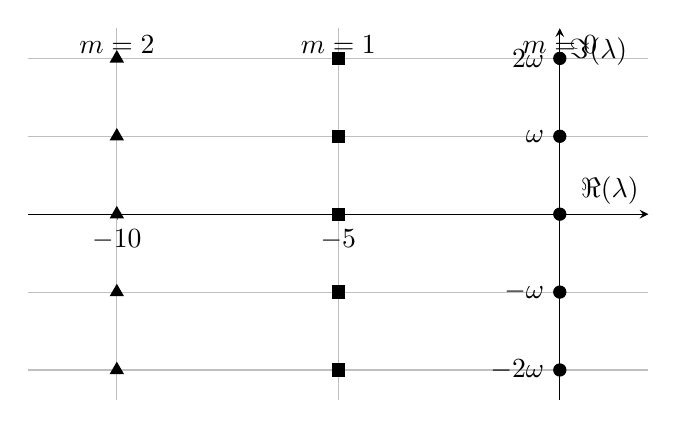
\begin{tikzpicture}
\begin{axis}[
    width=0.78\textwidth,
    height=0.52\textwidth,
    xlabel={$\Re(\lambda)$},
    ylabel={$\Im(\lambda)$},
    axis lines=middle,
    xmin=-12, xmax=2,
    ymin=-900, ymax=900,
    xtick={-10,-5,0},
    ytick={-754,-377,0,377,754},
    yticklabels={$-2\omega$,$-\omega$,0,$\omega$,$2\omega$},
    grid=both,
    enlargelimits=false,
]
% m=0
\addplot[
    only marks,
    mark=*,
    mark size=2.2pt
] coordinates {
    (0,-754) (0,-377) (0,0) (0,377) (0,754)
};

% m=1
\addplot[
    only marks,
    mark=square*,
    mark size=2.2pt
] coordinates {
    (-5,-754) (-5,-377) (-5,0) (-5,377) (-5,754)
};

% m=2
\addplot[
    only marks,
    mark=triangle*,
    mark size=2.6pt
] coordinates {
    (-10,-754) (-10,-377) (-10,0) (-10,377) (-10,754)
};

% labels
\node at (axis cs:0,820) {$m=0$};
\node at (axis cs:-5,820) {$m=1$};
\node at (axis cs:-10,820) {$m=2$};
\end{axis}
\end{tikzpicture}
\caption{Retícula espectral de Koopman para el ejemplo numérico con \(\omega\approx 377\ \text{rad/s}\) y \(\mu=-5\). Los círculos corresponden a \(m=0\), los cuadrados a \(m=1\) y los triángulos a \(m=2\), según \(\lambda_{k,m}=jk\omega-5m\).}
\label{fig:Koopman_ladder_numeric}
\end{figure}
La estructura descrita por \eqref{eq:Koopman_ladder_numeric_family} puede visualizarse como una retícula discreta en el plano complejo, en la que los armónicos de fase generan columnas verticales y los exponentes transversales introducen desplazamientos horizontales.
\subsection{Un ejemplo desarrollado: de una escalera exacta a una aproximación EDMD}

El ejemplo anterior muestra la retícula espectral como una colección de puntos en el plano complejo. Conviene ahora desarrollar con más detalle el puente entre esa estructura ideal y una aproximación computacional basada en datos. La idea será avanzar en dos pasos. Primero estudiaremos un modelo radial--fase en el que la escalera espectral aparece de manera exacta. Después tomaremos el oscilador de Duffing forzado como laboratorio numérico, donde las coordenadas y eigenfunciones de Koopman ya no están disponibles de forma cerrada y deben aproximarse mediante un diccionario finito de observables.

\paragraph{Un modelo radial--fase con espectro explícito.}
Consideremos un sistema escrito directamente en coordenadas de fase y amplitud transversal:
\begin{equation}
\dot{\rho}=-\sigma \rho,
\qquad
\dot{\theta}=\omega,
\qquad \sigma>0.
\label{eq:Koopman_radial_phase_model}
\end{equation}
La variable \(\theta\) describe el avance longitudinal sobre el ciclo límite, mientras que \(\rho\) mide la distancia transversal al ciclo. Si \(\rho=0\), el movimiento permanece sobre el ciclo. Si \(\rho\neq 0\), la trayectoria se aproxima al ciclo con tasa \(\sigma\).

Para construir observables adaptados a esta geometría, definimos
\begin{equation}
\phi_{k,m}(\rho,\theta)=\rho^m e^{jk\theta},
\qquad
k\in\mathbb{Z},\quad m\in\mathbb{N}_0.
\label{eq:Koopman_radial_phase_observable}
\end{equation}
El generador de Koopman para el sistema \eqref{eq:Koopman_radial_phase_model} es
\begin{equation}
\mathcal{K}g
=
\frac{\partial g}{\partial \rho}(-\sigma\rho)
+
\frac{\partial g}{\partial \theta}\omega.
\label{eq:Koopman_radial_phase_generator}
\end{equation}
Aplicándolo a \(\phi_{k,m}\), se obtiene
\begin{align}
\mathcal{K}\phi_{k,m}
&=
(-\sigma\rho)\,m\rho^{m-1}e^{jk\theta}
+
\omega\,(jk)\rho^m e^{jk\theta}
\\[1mm]
&=
(-m\sigma+jk\omega)\rho^m e^{jk\theta}.
\end{align}
Por tanto,
\begin{equation}
\mathcal{K}\phi_{k,m}
=
\lambda_{k,m}\phi_{k,m},
\qquad
\lambda_{k,m}=-m\sigma+jk\omega.
\label{eq:Koopman_radial_phase_ladder_exact}
\end{equation}
Esta es la escalera espectral en su forma más limpia. El índice \(k\) enumera los armónicos de fase; el índice \(m\) enumera las potencias de la coordenada transversal. La parte imaginaria proviene de la rotación sobre el ciclo y la parte real proviene de la contracción transversal.

La evolución de cada observable queda entonces dada por
\begin{equation}
\phi_{k,m}(\rho(t),\theta(t))
=
e^{(-m\sigma+jk\omega)t}\phi_{k,m}(\rho_0,\theta_0).
\label{eq:Koopman_radial_phase_evolution_exact}
\end{equation}
Esta expresión deja ver con claridad la interpretación geométrica discutida al inicio del capítulo: la exponencial temporal se conserva, pero su amplitud y fase quedan ponderadas por el observable geométrico evaluado en la condición inicial.

\paragraph{Duffing forzado como laboratorio numérico.}
El modelo radial--fase es útil porque permite derivar la estructura exacta. En problemas físicos, sin embargo, las coordenadas \(\rho\), \(\theta\) y las eigenfunciones de Koopman rara vez están disponibles de forma explícita. Para ilustrar la situación computacional, consideremos el oscilador de Duffing forzado:
\begin{equation}
\ddot{x}+\delta\dot{x}+\alpha x+\beta x^3=\gamma\cos(\Omega t).
\label{eq:Koopman_duffing_forced_second_order}
\end{equation}
Introduciendo \(v=\dot{x}\) y una fase externa \(\theta\), con \(\dot{\theta}=\Omega\), se obtiene el sistema autónomo extendido
\begin{equation}
\dot{x}=v,
\qquad
\dot{v}=-\delta v-\alpha x-\beta x^3+\gamma\cos\theta,
\qquad
\dot{\theta}=\Omega.
\label{eq:Koopman_duffing_autonomous}
\end{equation}
Para valores moderados de los parámetros, por ejemplo
\begin{equation}
\delta=0.2,
\qquad
\alpha=1,
\qquad
\beta=0.1,
\qquad
\gamma=0.3,
\qquad
\Omega=1,
\label{eq:Koopman_duffing_parameters}
\end{equation}
la respuesta estacionaria es periódica o casi periódica con una estructura armónica inducida por la excitación y por la no linealidad cúbica. A diferencia del modelo radial--fase, aquí no partimos de eigenfunciones conocidas. Lo que hacemos es seleccionar observables y aproximar la acción del operador de Koopman sobre el subespacio generado por ellos.

\paragraph{Diccionario de observables y cierre aproximado.}
Un diccionario razonable para el sistema \eqref{eq:Koopman_duffing_autonomous} puede incluir monomios en \(x\) y \(v\), junto con funciones trigonométricas de la fase de excitación:
\begin{equation}
\Psi(x,v,\theta)=
\begin{bmatrix}
1 & x & v & x^2 & xv & v^2 & x^3 & x^2v & xv^2 & v^3 &
\cos\theta & \sin\theta & x\cos\theta & x\sin\theta & v\cos\theta & v\sin\theta
\end{bmatrix}^{T}.
\label{eq:Koopman_duffing_dictionary}
\end{equation}
La elección no es única. Es una decisión de modelado. Si el diccionario es demasiado pobre, la aproximación no captura la estructura no lineal; si es demasiado grande, puede volverse mal condicionada o sobreajustada. En este sentido, la aproximación finita de Koopman siempre contiene una tensión entre expresividad, estabilidad numérica e interpretación física.

El cierre exacto no ocurre en general. Por ejemplo,
\begin{equation}
\mathcal{K}x=v,
\label{eq:Koopman_duffing_Kx}
\end{equation}
pero
\begin{equation}
\mathcal{K}v=-\delta v-\alpha x-\beta x^3+\gamma\cos\theta.
\label{eq:Koopman_duffing_Kv}
\end{equation}
Hasta aquí el diccionario anterior contiene los términos requeridos. Sin embargo, al aplicar el generador a observables como \(xv\) aparece
\begin{align}
\mathcal{K}(xv)
&=\dot{x}v+x\dot{v}
\\
&=v^2-\delta xv-\alpha x^2-\beta x^4+\gamma x\cos\theta.
\label{eq:Koopman_duffing_Kxv}
\end{align}
El término \(x^4\) muestra que el subespacio generado por el diccionario no es invariante bajo el generador. Por eso EDMD no debe interpretarse como una representación exacta, sino como una proyección aproximada de la acción de Koopman sobre un espacio finito de observables.

\paragraph{Ajuste matricial.}
Supongamos que se genera una trayectoria muestreada
\begin{equation}
z_k=(x_k,v_k,\theta_k),
\qquad k=0,1,\ldots,N.
\end{equation}
Evaluamos el diccionario en cada muestra y formamos las matrices
\begin{equation}
X=
\begin{bmatrix}
\Psi(z_0) & \Psi(z_1) & \cdots & \Psi(z_{N-1})
\end{bmatrix},
\qquad
Y=
\begin{bmatrix}
\Psi(z_1) & \Psi(z_2) & \cdots & \Psi(z_N)
\end{bmatrix}.
\label{eq:Koopman_duffing_XY}
\end{equation}
EDMD busca una matriz \(K\) tal que
\begin{equation}
Y\approx KX.
\label{eq:Koopman_duffing_EDMD_fit}
\end{equation}
La solución de mínimos cuadrados se escribe
\begin{equation}
K=YX^{\dagger},
\label{eq:Koopman_duffing_K_matrix}
\end{equation}
donde \(X^{\dagger}\) denota la pseudoinversa de \(X\). Esta matriz \(K\) aproxima el operador de Koopman discreto asociado al paso de muestreo \(\Delta t\):
\begin{equation}
\Psi(z_{k+1})\approx K\Psi(z_k).
\label{eq:Koopman_duffing_discrete_evolution}
\end{equation}

\paragraph{Lectura de eigenvalores y modos.}
Si \(\mu_j\) es un eigenvalor de la matriz discreta \(K\), entonces se relaciona formalmente con un exponente continuo mediante
\begin{equation}
\mu_j\approx e^{\lambda_j\Delta t},
\qquad
\lambda_j\approx \frac{\log(\mu_j)}{\Delta t}.
\label{eq:Koopman_duffing_discrete_to_continuous}
\end{equation}
Las partes imaginarias de \(\lambda_j\) revelan frecuencias observables, mientras que las partes reales indican crecimiento, decaimiento o persistencia dentro del subespacio de observables elegido. En el Duffing forzado, si la respuesta estacionaria está dominada por la excitación \(\Omega\), es natural esperar contribuciones cercanas a
\begin{equation}
\pm \Omega,
\qquad
\pm 2\Omega,
\qquad
\pm 3\Omega,
\qquad \ldots
\end{equation}
La no linealidad cúbica y la elección del diccionario determinan qué armónicos aparecen con mayor claridad.

\paragraph{Interpretación física.}
Este ejemplo permite separar tres niveles de lectura. En el modelo radial--fase, la escalera espectral aparece exactamente porque las coordenadas están adaptadas al ciclo límite. En el Duffing forzado, las coordenadas adaptadas no se conocen y se recurre a un diccionario de observables. EDMD construye entonces una matriz finita que aproxima la evolución de esos observables.

La diferencia con Fourier es importante. Fourier analiza una señal ya producida, por ejemplo \(x(t)\), y pregunta qué frecuencias contiene. Koopman pregunta por funciones del estado que evolucionan exponencialmente bajo el flujo. Por eso, Koopman no reemplaza a Fourier; lo extiende hacia observables dependientes del estado. En una señal de salida, ambas lecturas pueden encontrarse: Fourier revela el contenido espectral temporal, mientras que Koopman intenta relacionar ese contenido con la geometría del sistema dinámico que lo produce.

\PerspectivaComputacional{El notebook asociado a esta ventana puede simular el Duffing forzado, construir el diccionario \(\Psi\), formar las matrices \(X\) y \(Y\), calcular \(K=YX^\dagger\), comparar la predicción de \(x(t)\) y visualizar los eigenvalores discretos de Koopman junto con el espectro de Fourier de la señal.}

\subsection{Preparación para la geometría local}

La estructura espectral obtenida en esta sección pide ahora una interpretación geométrica más precisa. ¿Qué son exactamente esas direcciones transversales? ¿Cómo se organizan cerca del ciclo? ¿Qué tipo de coordenadas hacen visible la separación entre fase y amplitudes transversales?

Responder estas preguntas exige introducir una descripción local de la vecindad del ciclo límite. Ese será el tema de la siguiente sección, donde examinaremos la geometría de fase y la idea de \emph{tube straightening}.
\section{Coordenadas de fase y \emph{tube straightening}}

La escalera espectral de la sección anterior sugirió que, cerca de un ciclo límite, la dinámica puede descomponerse en dos ingredientes: una evolución longitudinal a lo largo de la órbita, organizada por la fase, y una evolución transversal asociada a decaimientos o crecimientos respecto del ciclo. Para que esta descomposición no permanezca solo como una intuición espectral, conviene introducir una imagen geométrica precisa. Esa imagen es la de una vecindad tubular alrededor del ciclo límite y su enderezamiento local, lo que en este contexto llamaremos \emph{tube straightening}.

\subsection{La vecindad tubular del ciclo límite}
\begin{figure}[t]
\centering
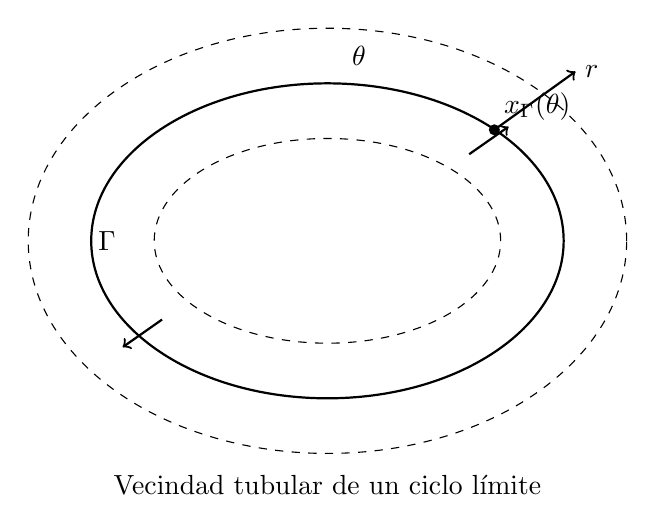
\begin{tikzpicture}[scale=1.0]
    % ciclo límite
    \draw[thick] (0,0) ellipse (3 and 2);

    % vecindad tubular
    \draw[dashed] (0,0) ellipse (3.8 and 2.7);
    \draw[dashed] (0,0) ellipse (2.2 and 1.3);

    % flechas sobre el ciclo (segmentos simples para evitar problemas)
    \draw[->,thick] (1.8,1.1) -- (2.3,1.45);
    \draw[->,thick] (-2.1,-1.0) -- (-2.6,-1.35);

    % punto sobre el ciclo
    \fill (2.12,1.41) circle (2pt);
    \node[above right] at (2.12,1.41) {$x_{\Gamma}(\theta)$};

    % dirección transversal
    \draw[->,thick] (2.12,1.41) -- (3.15,2.15);
    \node[right] at (3.15,2.15) {$r$};

    % etiquetas
    \node at (0.4,2.35) {$\theta$};
    \node at (-2.8,0) {$\Gamma$};
    \node at (0,-3.1) {Vecindad tubular de un ciclo l\'imite};
\end{tikzpicture}
\caption{Ciclo l\'imite \(\Gamma\) y su vecindad tubular. La coordenada longitudinal est\'a dada por la fase \(\theta\), mientras que \(r\) representa una coordenada transversal local.}
\label{fig:koopman_tube_neighborhood}
\end{figure}
Sea \(\Gamma\) un ciclo límite suave de período \(T\) para el sistema
\begin{equation}
\dot{x}=f(x),
\label{eq:Koopman_tube_system}
\end{equation}
y sea \(\omega=2\pi/T\) su frecuencia angular. En una vecindad suficientemente pequeña de \(\Gamma\), es natural pensar el espacio de estados como organizado alrededor de la órbita periódica, del mismo modo que una curva suave admite una vecindad tubular en geometría diferencial.

De manera intuitiva, cada punto cercano a \(\Gamma\) puede describirse mediante:
\begin{itemize}
\item una coordenada longitudinal, que indica la posición relativa sobre el ciclo;
\item y una o varias coordenadas transversales, que indican la desviación respecto de la órbita.
\end{itemize}
La coordenada longitudinal será la fase \(\theta\), mientras que las coordenadas transversales capturarán la aproximación o alejamiento del ciclo.

\subsection{Coordenadas de fase}
\begin{figure}[t]
\centering
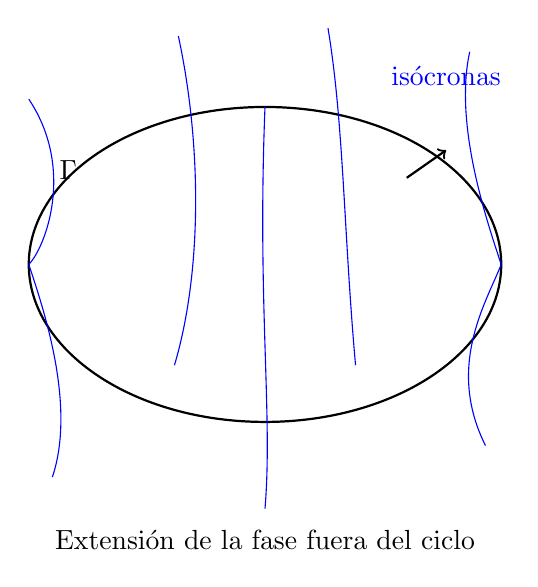
\begin{tikzpicture}[scale=1.0]
    % ciclo límite
    \draw[thick] (0,0) ellipse (3 and 2);

    % isócronas estilizadas
    \draw[blue] (2.6,2.7) .. controls (2.4,1.8) and (2.8,0.6) .. (3,0);
    \draw[blue] (0.8,3.0) .. controls (1.0,1.8) and (1.0,0.4) .. (1.15,-1.28);
    \draw[blue] (-1.1,2.9) .. controls (-0.8,1.5) and (-0.8,-0.1) .. (-1.15,-1.28);
    \draw[blue] (-3.0,2.1) .. controls (-2.4,1.2) and (-2.8,0.2) .. (-3.0,0);
    \draw[blue] (-2.7,-2.7) .. controls (-2.4,-1.8) and (-2.8,-0.6) .. (-3.0,0);
    \draw[blue] (0.0,-3.1) .. controls (0.1,-1.9) and (-0.1,-0.5) .. (0,2);
    \draw[blue] (2.8,-2.3) .. controls (2.3,-1.3) and (2.8,-0.5) .. (3,0);

    % flecha sobre el ciclo
    \draw[->,thick] (1.8,1.1) -- (2.3,1.45);

    % etiquetas
    \node at (-2.5,1.2) {$\Gamma$};
    \node[blue] at (2.3,2.4) {is\'ocronas};
    \node at (0,-3.5) {Extensi\'on de la fase fuera del ciclo};
\end{tikzpicture}
\caption{Esquema de is\'ocronas alrededor de un ciclo l\'imite. Cada curva re\'une puntos con la misma fase asint\'otica \(\theta\).}
\label{fig:koopman_isochrones}
\end{figure}

La fase asintótica ya introducida en la sección anterior proporciona la coordenada natural a lo largo de la órbita:
\begin{equation}
\theta:X\to \mathbb{R}/2\pi\mathbb{Z},
\label{eq:Koopman_tube_phase}
\end{equation}
con evolución
\begin{equation}
\theta(\varphi^t(x))=\theta(x)+\omega t
\quad \text{mod } 2\pi.
\label{eq:Koopman_tube_phase_evolution}
\end{equation}
Sobre el ciclo mismo, esta coordenada recorre uniformemente la órbita. En una vecindad atractora, las superficies de fase constante forman las isócronas, que actúan como hojas de una foliación local alrededor del ciclo.

Desde esta perspectiva, la fase no es solo una parametrización conveniente de la órbita, sino una coordenada geométrica que organiza toda una vecindad del ciclo límite.

\subsection{Coordenadas transversales}

Además de la fase, se requieren coordenadas que midan la separación respecto del ciclo. Denotemos de manera genérica estas coordenadas por
\begin{equation}
r=(r_1,\dots,r_q),
\label{eq:Koopman_tube_transverse_coords}
\end{equation}
donde \(q=n-1\) en el caso más simple de una órbita periódica aislada en un sistema de dimensión \(n\). Cerca del ciclo, puede pensarse que cada \(r_i\) describe una amplitud transversal asociada a una dirección característica de aproximación o repulsión.

En coordenadas locales \((\theta,r)\), la dinámica cerca del ciclo límite puede representarse esquemáticamente como
\begin{equation}
\dot{\theta}=\omega+\text{correcciones},
\label{eq:Koopman_tube_theta_dynamics}
\end{equation}
\begin{equation}
\dot{r}=B(\theta)r+\text{términos de orden superior},
\label{eq:Koopman_tube_r_dynamics}
\end{equation}
donde \(B(\theta)\) es una matriz periódica en \(\theta\). Esta forma deja ver con claridad la separación entre la dinámica longitudinal y la transversal.

\subsection{El sentido del \emph{tube straightening}}
\begin{figure}[t]
\centering
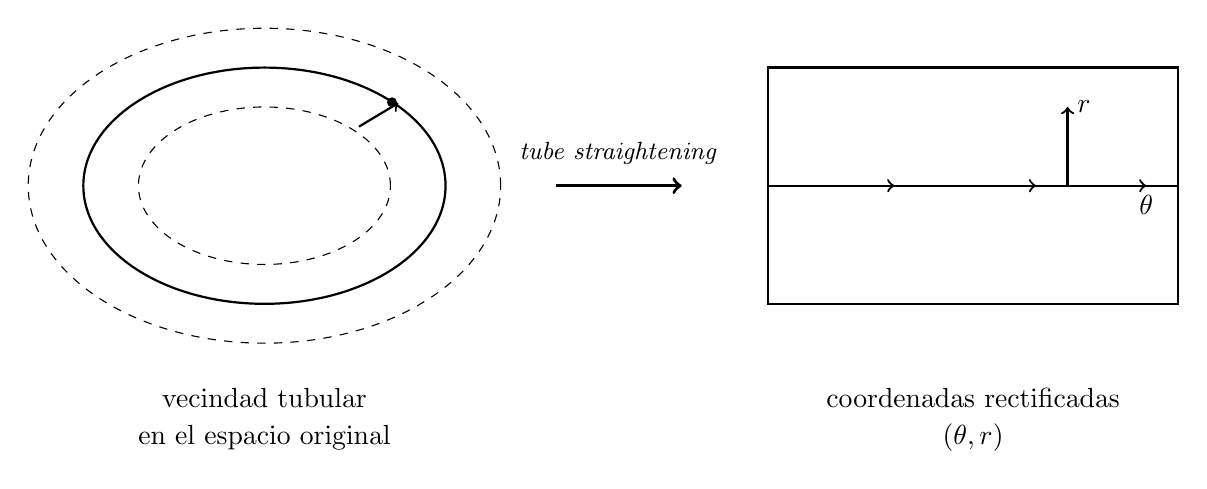
\begin{tikzpicture}[scale=1.0]

    % izquierda: tubo curvo
    \begin{scope}[shift={(-4.5,0)}]
        \draw[thick] (0,0) ellipse (2.3 and 1.5);
        \draw[dashed] (0,0) ellipse (3.0 and 2.0);
        \draw[dashed] (0,0) ellipse (1.6 and 1.0);

        \draw[->,thick] (1.2,0.75) -- (1.7,1.05);
        \fill (1.62,1.06) circle (1.8pt);

        \node at (0,-2.7) {vecindad tubular};
        \node at (0,-3.2) {en el espacio original};
    \end{scope}

    % flecha central
    \draw[->,very thick] (-0.8,0) -- (0.8,0);
    \node[above] at (0,0.15) {\small \emph{tube straightening}};

    % derecha: coordenadas rectificadas
    \begin{scope}[shift={(4.5,0)}]
        \draw[thick] (-2.6,-1.5) rectangle (2.6,1.5);

        % línea central
        \draw[thick] (-2.6,0) -- (2.6,0);

        % flechas longitudinales
        \draw[->,thick] (-1.8,0) -- (-1.0,0);
        \draw[->,thick] (0.0,0) -- (0.8,0);
        \draw[->,thick] (1.4,0) -- (2.2,0);

        % coordenada transversal
        \draw[->,thick] (1.2,0) -- (1.2,1.0);
        \node[right] at (1.2,1.0) {$r$};

        % etiqueta theta
        \node[below] at (2.2,0) {$\theta$};

        \node at (0,-2.7) {coordenadas rectificadas};
        \node at (0,-3.2) {$(\theta,r)$};
    \end{scope}

\end{tikzpicture}
\caption{Idea geom\'etrica del \emph{tube straightening}. A la izquierda, una vecindad tubular alrededor del ciclo l\'imite en el espacio original. A la derecha, una representaci\'on local rectificada donde la din\'amica se separa en una direcci\'on de fase \(\theta\) y coordenadas transversales \(r\).}
\label{fig:koopman_tube_straightening}
\end{figure}
La expresión \eqref{eq:Koopman_tube_theta_dynamics}--\eqref{eq:Koopman_tube_r_dynamics} ya es útil, pero todavía conserva la modulación periódica explícita en la dependencia de \(B(\theta)\). La idea de \emph{tube straightening} consiste en buscar coordenadas locales mejor adaptadas al ciclo límite, en las cuales la vecindad tubular se enderece y la dinámica se separe de manera más transparente en:
\begin{enumerate}
\item una rotación uniforme en la coordenada de fase;
\item una dinámica transversal aproximadamente lineal.
\end{enumerate}

En otras palabras, se busca un sistema de coordenadas en el que el ciclo límite mismo quede representado por
\[
r=0,
\]
y la evolución longitudinal sea simplemente
\[
\dot{\theta}=\omega.
\]
Las coordenadas transversales quedan entonces organizadas alrededor de esa columna central, como si se hubiera ``enderezado'' la vecindad del ciclo.

\subsection{Forma local rectificada}

En una formulación idealizada, la dinámica local rectificada cerca del ciclo puede escribirse como
\begin{equation}
\dot{\theta}=\omega,
\label{eq:Koopman_tube_straight_theta}
\end{equation}
\begin{equation}
\dot{r}=\Lambda r+\text{términos no lineales y acoplados},
\label{eq:Koopman_tube_straight_r}
\end{equation}
donde \(\Lambda\) es una matriz constante o, al menos, una matriz que captura la dinámica transversal principal. Si el ciclo es estable, los autovalores de \(\Lambda\) tendrán parte real negativa.

Esta forma local ya sugiere de manera muy directa la estructura espectral de Koopman:
\begin{itemize}
\item la ecuación \(\dot{\theta}=\omega\) produce los armónicos \(e^{jk\theta}\) con autovalores \(jk\omega\);
\item la ecuación transversal \(\dot{r}=\Lambda r\) produce factores exponenciales asociados a los autovalores transversales;
\item y la combinación de ambos genera la escalera espectral descrita antes.
\end{itemize}

\subsection{Geometría y espectro}

La importancia de esta rectificación local es que une geometría y espectro en una sola imagen. La fase proporciona la dirección tangencial a la órbita; las coordenadas transversales proporcionan direcciones de alejamiento o aproximación; y la teoría de Koopman traduce esas dos piezas geométricas en eigenfunciones y autovalores.

Así, la estructura
\[
jk\omega+\sum_r m_r\mu_r
\]
no debe verse como una combinación algebraica arbitraria. Es la traducción espectral de una geometría local rectificada alrededor del ciclo límite: rotación uniforme en la dirección de fase y evolución exponencial en las direcciones transversales.

\subsection{Relación con Floquet}

La proximidad con la teoría de Floquet se vuelve aquí especialmente evidente. En Floquet, la linealización periódica alrededor del ciclo producía exponentes transversales modulados por la periodicidad. En la formulación geométrica actual, el \emph{tube straightening} organiza esa misma información en coordenadas locales donde la fase y la transversalidad quedan separadas.

Podría decirse que Floquet ofrece la lectura lineal periódica de la vecindad del ciclo, mientras que Koopman ofrece la lectura sobre observables de esa misma estructura. Ambas teorías están, por tanto, mirando el mismo fenómeno desde lados diferentes:
\begin{itemize}
\item Floquet desde la dinámica linealizada en el espacio tangente;
\item Koopman desde la evolución lineal sobre funciones del estado.
\end{itemize}

\subsection{Interpretación para oscilaciones}

En el análisis de oscilaciones, esta geometría local resulta especialmente valiosa. Permite entender un régimen periódico no solo como una órbita en el espacio de estados, sino como una estructura organizada por:
\begin{itemize}
\item una frecuencia básica de rotación;
\item decaimientos o crecimientos transversales;
\item y observables que pueden alinearse con esas dos formas de evolución.
\end{itemize}

En sistemas eléctricos de potencia, esta lectura puede ser particularmente útil cuando se desea distinguir entre:
\begin{enumerate}
\item la periodicidad principal de operación;
\item modulaciones armónicas o subarmónicas;
\item y modos transversales asociados a estabilidad local o amortiguamiento.
\end{enumerate}
La geometría local del ciclo y su lectura espectral ayudan así a organizar la interpretación de oscilaciones complejas sin perder el vínculo con cantidades físicamente observables.

\subsection{Puente hacia observables armónicos}

La rectificación local también prepara el paso a la siguiente sección. Una vez introducidas coordenadas \((\theta,r)\) cerca del ciclo, se vuelve natural construir observables que dependan armónicamente de la fase y funcionalmente de las coordenadas transversales. Esa será precisamente la conexión con observables armónicos:
\[
e^{jk\theta},\qquad
e^{jk\theta}\psi(r),\qquad
e^{jk\theta}\psi_1(r)^{m_1}\cdots\psi_q(r)^{m_q}.
\]
Allí la teoría de Koopman mostrará con toda claridad cómo la estructura geométrica local se traduce en una familia organizada de observables espectrales.

\subsection{Cierre de la sección}

La noción de \emph{tube straightening} da, por tanto, una base geométrica precisa a la escalera espectral de Koopman. La fase organiza la dirección longitudinal; las coordenadas transversales organizan la estabilidad local; y la rectificación de la vecindad del ciclo convierte ambas piezas en una estructura compatible con una lectura espectral lineal sobre observables. En este punto, la fase ya no es solo una herramienta de parametrización, sino el eje de una geometría local que prepara directamente la expansión en observables armónicos.
\section{Conexión con observables armónicos}

Las secciones anteriores mostraron que, cerca de un ciclo límite, la dinámica puede organizarse geométricamente en una coordenada de fase \(\theta\) y en un conjunto de coordenadas transversales \(r\). También vimos que esta separación induce una estructura espectral de Koopman formada por armónicos de fase y exponentes transversales. Conviene ahora dar un paso adicional y examinar cómo esta arquitectura se refleja directamente en los observables.

La idea central es la siguiente: una vez que la vecindad del ciclo ha sido descrita en coordenadas \((\theta,r)\), resulta natural construir observables que dependan armónicamente de la fase y funcionalmente de las coordenadas transversales. Estos observables forman una familia particularmente bien adaptada a la dinámica periódica local y permiten traducir la geometría del ciclo límite en una expansión espectral explícita.

\subsection{Observables armónicos de fase}

El caso más simple es el de los observables puramente armónicos en la fase,
\begin{equation}
g_k(x)=e^{jk\theta(x)},
\qquad
k\in\mathbb{Z}.
\label{eq:Koopman_harmonic_observables_phase}
\end{equation}
Como se vio antes, estas funciones son eigenfunciones de Koopman asociadas a los autovalores
\begin{equation}
\lambda_k=jk\omega.
\label{eq:Koopman_harmonic_observables_phase_eigs}
\end{equation}
Sobre el ciclo límite, esta familia desempeña el papel de una base de Fourier adaptada al flujo. En efecto, si \(g\) es un observable suficientemente regular restringido a la órbita periódica, entonces puede expandirse como
\begin{equation}
g|_{\Gamma}(\theta)=\sum_{k\in\mathbb{Z}}\hat{g}_k e^{jk\theta}.
\label{eq:Koopman_harmonic_observables_fourier}
\end{equation}

Esta fórmula muestra que la expansión de Fourier clásica reaparece aquí de manera natural, pero ahora expresada no como función del tiempo directamente, sino como función de la fase geométrica del ciclo límite. La periodicidad ya no está impuesta externamente por el tiempo, sino internalizada en una coordenada del flujo.

\subsection{Observables mixtos: fase y transversalidad}

La familia \eqref{eq:Koopman_harmonic_observables_phase} captura únicamente la dinámica longitudinal. Para describir también la estructura transversal, es natural considerar observables del tipo
\begin{equation}
g(\theta,r)=e^{jk\theta}\,\psi(r),
\label{eq:Koopman_harmonic_observables_mixed}
\end{equation}
donde \(\psi(r)\) es una función de las coordenadas transversales. Si \(\psi\) está asociada a una eigenfunción transversal de Koopman con autovalor \(\mu\), entonces el observable total evoluciona con autovalor
\begin{equation}
\lambda=jk\omega+\mu.
\label{eq:Koopman_harmonic_observables_mixed_eig}
\end{equation}
Más generalmente, si hay varias coordenadas transversales y varias funciones propias \(\psi_1,\dots,\psi_q\), puede considerarse la familia
\begin{equation}
g_{k,\mathbf{m}}(x)
=
e^{jk\theta(x)}
\psi_1(x)^{m_1}\cdots\psi_q(x)^{m_q},
\label{eq:Koopman_harmonic_observables_general}
\end{equation}
con autovalores
\begin{equation}
\lambda_{k,\mathbf{m}}
=
jk\omega+\sum_{r=1}^{q}m_r\mu_r.
\label{eq:Koopman_harmonic_observables_general_eig}
\end{equation}

Esta construcción deja ver con total claridad el papel de los observables armónicos: no son solo funciones convenientes, sino portadores directos de la estructura espectral local del sistema.

\subsection{Relación con Fourier}

El vínculo con Fourier merece destacarse. En una señal puramente periódica, la expansión
\[
\sum_k \hat{g}_k e^{jk\omega t}
\]
organiza la información en armónicos temporales. Cerca de un ciclo límite, la teoría de Koopman reemplaza esta descripción por una expansión en términos de la fase geométrica:
\[
\sum_k \hat{g}_k e^{jk\theta(x)}.
\]
La diferencia es profunda. En Fourier, el argumento es el tiempo. En Koopman, el argumento es una función del estado que evoluciona linealmente a lo largo del flujo.

Esto convierte a los armónicos de fase en una suerte de Fourier intrínseco del sistema alrededor del ciclo límite. La expansión deja de ser puramente temporal y pasa a ser dinámica y geométrica a la vez.

\subsection{Relación con Floquet}

La conexión con Floquet también se vuelve ahora más precisa. En Floquet, una solución de un sistema lineal periódico podía escribirse como
\[
p(t)e^{\rho t},
\]
donde \(p(t)\) era periódica. Al expandir \(p(t)\) en Fourier, aparecían familias de exponentes desplazados por \(jk\omega\). En Koopman, la misma lógica reaparece, pero ahora codificada directamente en observables:
\[
e^{jk\theta(x)}\psi(x),
\]
con autovalores
\[
jk\omega+\mu.
\]

Podría decirse que Floquet describe una modulación periódica sobre modos del espacio tangente, mientras que Koopman describe una modulación armónica sobre funciones del estado. La cercanía estructural entre ambas teorías es una de las razones por las que este capítulo se sitúa naturalmente después del de Floquet.

\subsection{Relación con Carleman}

También aquí puede verse un vínculo con Carleman. En el \emph{embedding} de Carleman, los observables monomiales daban lugar a una estructura lineal infinita-dimensional adaptada a la no linealidad polinomial. En el caso actual, los observables armónicos de fase y sus combinaciones con funciones transversales generan una estructura lineal adaptada a la geometría periódica local.

Esta comparación es importante porque muestra que la teoría de Koopman no reemplaza simplemente a Carleman, sino que amplía el horizonte. Allí donde Carleman privilegiaba monomios del estado, Koopman permite incorporar familias de observables más generales, incluyendo armónicos de fase, observables isostables y combinaciones funcionales más cercanas a la estructura real del flujo.

\subsection{Interpretación para observables físicos}

Desde el punto de vista aplicado, esta formulación es especialmente útil porque los observables que interesan en la práctica rara vez son las coordenadas del estado puras. En sistemas eléctricos de potencia, por ejemplo, pueden ser más relevantes tensiones, corrientes, potencias, ángulos relativos, salidas medidas o variables agregadas. La teoría de Koopman sugiere que, cerca de un ciclo límite, tales cantidades pueden descomponerse en contribuciones armónicas y transversales organizadas por la estructura espectral local.

Esto proporciona una forma especialmente rica de interpretar señales oscilatorias. En lugar de ver una medición como una simple mezcla temporal de frecuencias, se la puede entender como proyección de la dinámica sobre una familia de observables armónicamente organizados. La señal observada se convierte así en ventana hacia la geometría local del flujo.

\subsection{Una expansión local adaptada al ciclo}

De manera esquemática, un observable regular \(g(x)\) cerca del ciclo límite puede pensarse como expandible en una familia del tipo
\begin{equation}
g(x)\approx \sum_{k,\mathbf{m}} c_{k,\mathbf{m}}\,
e^{jk\theta(x)}
\psi_1(x)^{m_1}\cdots\psi_q(x)^{m_q}.
\label{eq:Koopman_harmonic_observables_local_expansion}
\end{equation}
Esta expresión puede verse como una expansión local adaptada al ciclo, en la que:
\begin{itemize}
\item los factores \(e^{jk\theta(x)}\) organizan la periodicidad longitudinal;
\item las potencias de \(\psi_r(x)\) organizan la estructura transversal;
\item y los coeficientes \(c_{k,\mathbf{m}}\) dependen del observable físico considerado.
\end{itemize}

Desde esta perspectiva, la teoría de Koopman ofrece algo más que un conjunto de autovalores. Ofrece una gramática local para expandir observables alrededor de un ciclo límite.

\Advertencia{La expresión \eqref{eq:Koopman_harmonic_observables_local_expansion} debe leerse como una expansión local, formal o aproximada, adaptada a la vecindad del ciclo límite. No afirma que todo observable admita automáticamente una expansión global convergente de este tipo. Su valor principal, para nuestros fines, es organizar qué familias de funciones son naturalmente compatibles con la geometría periódica del flujo.}

\subsection{Cierre conceptual de la sección}

La conexión con observables armónicos completa la interpretación operatorial de la dinámica periódica local. La fase, las coordenadas transversales y la escalera espectral ya no aparecen como piezas separadas, sino como partes de una misma estructura funcional. La periodicidad se traduce en armónicos de fase; la estabilidad transversal se traduce en exponentes adicionales; y los observables físicos se organizan como combinaciones de ambos.

Con ello, la teoría de Koopman se revela como una síntesis especialmente poderosa de varias ideas que han atravesado esta monografía: Fourier reaparece como expansión en fase, Floquet como retícula espectral desplazada, y Carleman como linealidad sobre familias especiales de funciones del estado. Koopman reúne esas intuiciones en una formulación operatorial donde la dinámica se vuelve transparente no solo por sus trayectorias, sino por la evolución de los observables adecuados.

\section{Lectura computacional y advertencias prácticas}

La formulación anterior es conceptualmente poderosa, pero su uso computacional exige una advertencia inmediata: en la práctica no se dispone del espacio completo de observables. Se trabaja con una familia finita de funciones candidatas, con datos muestreados y con aproximaciones numéricas. Por eso, la teoría de Koopman debe leerse no solo como una teoría espectral exacta, sino también como una guía para construir representaciones finitas útiles.

\subsection{La elección de observables}

El paso decisivo en cualquier aproximación computacional de Koopman es la elección de observables. Si se escogen únicamente las coordenadas originales del estado, la representación puede perder la estructura que se desea revelar. Si se incluyen funciones más adaptadas a la dinámica —por ejemplo armónicos de fase, amplitudes transversales, productos entre fase e isostables, potencias o funciones no lineales de salidas físicas— la aproximación puede capturar mejor la organización local del ciclo límite.

Esta observación conecta directamente con la intuición de Carleman. Allí la familia de observables estaba dada por monomios. En Koopman, esa familia puede ampliarse: no solo monomios del estado, sino también observables geométricos, armónicos, energéticos o físicamente medibles. La calidad de una aproximación finita depende entonces de qué tan bien esa familia elegida represente la estructura que el sistema realmente usa para evolucionar.

\subsection{DMD y EDMD como aproximaciones finitas}

Métodos como DMD y EDMD pueden entenderse como intentos de aproximar una parte finita del operador de Koopman a partir de datos. DMD trabaja con observables muy cercanos a las coordenadas originales, mientras que EDMD permite ampliar el diccionario de observables. Desde la perspectiva de este capítulo, EDMD resulta especialmente natural cerca de ciclos límite, porque permite incluir funciones que imiten la forma esperada de la escalera espectral:
\[
e^{jk\theta},\qquad
\psi_r,\qquad
e^{jk\theta}\psi_r^m.
\]

La dificultad práctica es que la fase \(\theta\) y las coordenadas transversales \(\psi_r\) no siempre son conocidas. A veces deben estimarse a partir de datos, reconstruirse mediante embeddings de retardos, aproximarse mediante observables físicos o inferirse a partir de modelos. Por ello, la lectura computacional de Koopman no elimina el juicio del analista: lo desplaza hacia la construcción de un diccionario de observables significativo.

\subsection{Interpretación para señales medidas}

En aplicaciones de potencia, las señales disponibles suelen ser tensiones, corrientes, potencias, frecuencias locales, ángulos o magnitudes agregadas. Estas señales no revelan toda la dinámica interna, sino una proyección particular sobre observables medibles. La teoría de Koopman sugiere que una señal oscilatoria puede contener contribuciones de varios elementos de la retícula espectral: armónicos de fase, modos transversales amortiguados y combinaciones entre ambos.

Esto es importante porque una frecuencia observada en una medición no necesariamente corresponde a un modo aislado del espacio de estados. Puede ser la huella de un observable mixto, por ejemplo una componente armónica modulada por una dirección transversal. Bajo esta interpretación, el análisis espectral de señales deja de ser solo una lectura temporal y se convierte en una ventana parcial hacia la geometría local del flujo.

\subsection{Una ventana computacional natural}

Una ventana computacional especialmente adecuada para este capítulo consistiría en estudiar un oscilador normal en coordenadas polares,
\begin{equation}
\dot{r}=\sigma(1-r)r,
\qquad
\dot{\theta}=\omega,
\label{eq:Koopman_computational_window_normal_form}
\end{equation}
con \(\sigma>0\). El ciclo límite está dado por \(r=1\), la fase avanza uniformemente y la variable transversal \(r-1\) decae exponencialmente, al menos localmente. En este caso, los observables
\[
e^{jk\theta},
\qquad
(r-1)^m e^{jk\theta}
\]
permiten visualizar de manera directa la escalera
\[
\lambda_{k,m}=jk\omega-m\sigma.
\]

El valor pedagógico de este ejemplo es grande: permite graficar el ciclo límite, observar trayectorias que convergen hacia él, construir la retícula espectral y reconstruir señales con pocos observables armónicos y transversales. Sería una continuación natural de las ventanas computacionales anteriores, porque transforma la teoría operatorial en una experiencia visual y numérica.

\subsection{Cierre práctico}

La lección práctica puede resumirse así: Koopman ofrece un lenguaje lineal sobre observables, pero la utilidad de ese lenguaje depende de elegir observables que respeten la geometría del problema. Cerca de ciclos límite, la fase, los armónicos y las coordenadas transversales proporcionan una guía privilegiada. En aplicaciones reales, el reto consiste en aproximar esas funciones con los datos y mediciones disponibles, sin olvidar que toda representación finita es una ventana parcial sobre un operador mucho más amplio.


\section*{Conclusión}

Este capítulo mostró que la teoría de Koopman ofrece una de las formulaciones más amplias y sugerentes para estudiar la dinámica cerca de ciclos límite. Su movimiento conceptual fundamental consiste en desplazar el foco desde la evolución del estado hacia la evolución de observables. Con ello, una dinámica no lineal puede adquirir una representación lineal en un espacio funcional, y estructuras que en el espacio de estados aparecían mezcladas o implícitas se vuelven espectralmente visibles.

La introducción del operador y del generador de Koopman permitió fijar esta idea con precisión: la linealidad no se recupera en el espacio de estado original, sino en la acción inducida sobre funciones del estado. En ese marco, las eigenfunciones de fase revelaron que la periodicidad del ciclo límite puede traducirse en una familia de observables que evolucionan exponencialmente con autovalores \(jk\omega\). La fase dejó así de ser solo una coordenada geométrica y pasó a convertirse en estructura espectral.

La incorporación de direcciones transversales enriqueció esta imagen. Los exponentes asociados a la atracción o repulsión respecto del ciclo se combinaron con los armónicos de fase para producir una escalera espectral organizada por expresiones del tipo
\[
jk\omega+\sum_r m_r\mu_r.
\]
Esta fórmula mostró con claridad que la periodicidad y la estabilidad transversal no son rasgos separados, sino componentes de una misma arquitectura local. La geometría del ciclo límite, la teoría de Floquet y la lectura operatorial de Koopman convergieron así en una estructura común.

La discusión de coordenadas de fase y \emph{tube straightening} dio a esta estructura un fundamento geométrico más preciso. La vecindad del ciclo pudo entenderse como una región organizada por una dirección longitudinal de fase y varias direcciones transversales. La teoría de Koopman tradujo esta geometría en familias de observables armónicos y transversales, mostrando que la dinámica local puede expandirse en funciones adaptadas a la estructura del flujo.

La conexión con observables armónicos permitió finalmente reunir varias de las intuiciones que han atravesado esta monografía. Fourier reapareció como expansión en armónicos de fase; Floquet reapareció como organización de exponentes desplazados por la frecuencia base; Carleman reapareció como linealidad sobre familias especiales de funciones del estado. Koopman no sustituyó a estas teorías, sino que las reubicó dentro de un marco más general en el que la linealidad se formula sobre observables y no necesariamente sobre coordenadas del estado.

Visto en perspectiva, este capítulo culmina el hilo central de la Parte III. Floquet mostró cómo reorganizar la periodicidad lineal. Carleman mostró cómo desplegar la no linealidad polinomial en una cascada lineal infinita. Koopman mostró, finalmente, que la dinámica puede estudiarse desde el lado de las funciones que mejor revelan su estructura. El paso de estados a observables no fue un cambio meramente técnico, sino una ampliación del punto de vista.

Con ello, la monografía alcanza uno de sus mensajes más profundos: la dinámica periódica y débilmente no lineal no solo puede aproximarse, sino también reorganizarse de maneras conceptualmente fecundas. Armónicos, modos, liftings, monomios y observables han aparecido aquí no como técnicas aisladas, sino como distintas puertas de entrada a una misma intuición: la estructura emerge cuando se elige el espacio adecuado para mirar la dinámica.
